\documentclass{beamer}
\usetheme{Boadilla}


\title{Midterm Project}
\subtitle{Performance of explainer in different text classification models}
\author{Zexin Ren}
\date{\today}


\begin{document}



\begin{frame}
    \titlepage

\end{frame}

\section{Introduction}
\subsection{Explainer}
\subsection{Model and Dataset}
\section{Analysis Method}
\subsection{Salience Analysis}
\subsection{Top K Features Mask}


\section{Result}
\subsection{Accuracy Tendency}



\begin{frame}
    \frametitle{Outline}
    \tableofcontents
\end{frame}


\begin{frame}{Introduction}
\frametitle{Introduction}
\framesubtitle{Explainer}
"Why Should I Trust You?": Explaining the Predictions of Any Classifier
\begin{figure}
    \centering
        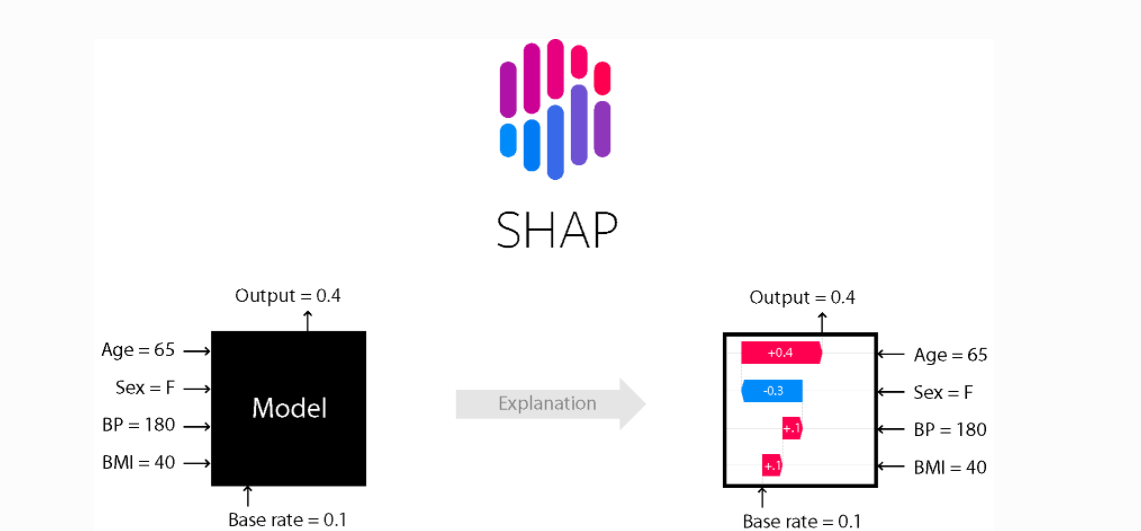
\includegraphics[width=0.7\textwidth]{ExplainerIntroduction.png}
        \caption{An example of SHAP explainer}
        \label{fig:ExplainerIntroduction}
    \end{figure}
\end{frame}

\begin{frame}
    \frametitle{Introduction}
    \framesubtitle{Model and Dataset}

    \begin{tabular}{|c||c||c|}
        \hline
             & Model 1 & Model 2 \\ 
        \hline
            Num. of Labels & 2 & 5\\ 
        \hline
            Model Name & distilbert-base-uncased & distilbert-base-uncased\\ 
        \hline
        Tokenizer Name & distilbert-base-uncased & distilbert-base-uncased\\ 
        \hline
        Dataset & Clinical Statement  & Medical abstracts \\ 
        \hline
        Test Accuracy & $85.5\%$ & $77\%$\\ 
        \hline
        \end{tabular}

\end{frame}


\begin{frame}
    \frametitle{Method}
    \framesubtitle{Salience Analysis}

    \begin{figure}
        \centering
            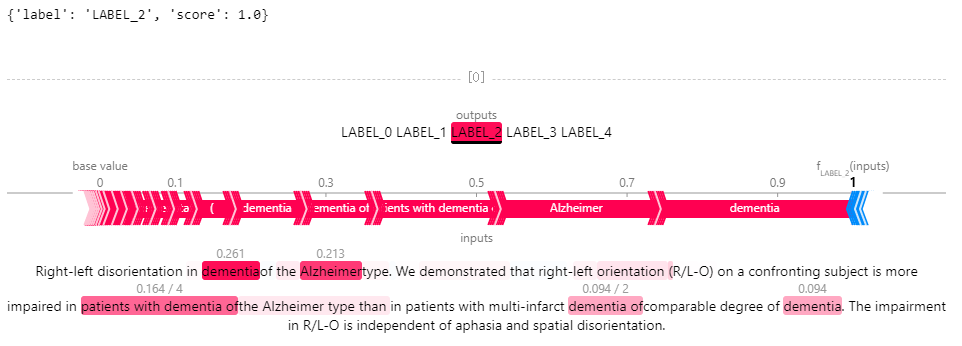
\includegraphics[width=1\textwidth]{Saliency Example4.png}
            \caption{A Text Example}
            \label{fig:TextExample}
        \end{figure}


\end{frame}

\begin{frame}
    \frametitle{Method}
    \framesubtitle{Top K Mask}
How to test this result?
    \begin{figure}
        \centering
            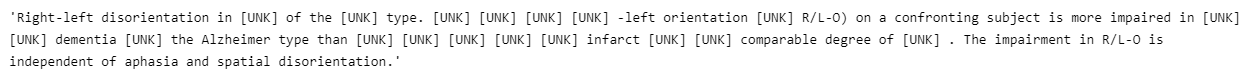
\includegraphics[width=1\textwidth]{Top K Masked3.png}
            \caption{Top K masked}
            \label{fig:MaskedExample}
    \end{figure}

\par
Repeat the same process to all sample on the test set, to see if the accuracy will decrease.
\end{frame}

\begin{frame}
    \frametitle{Result}
    \framesubtitle{Accuracy Tendency}
    \begin{figure}
        \centering
            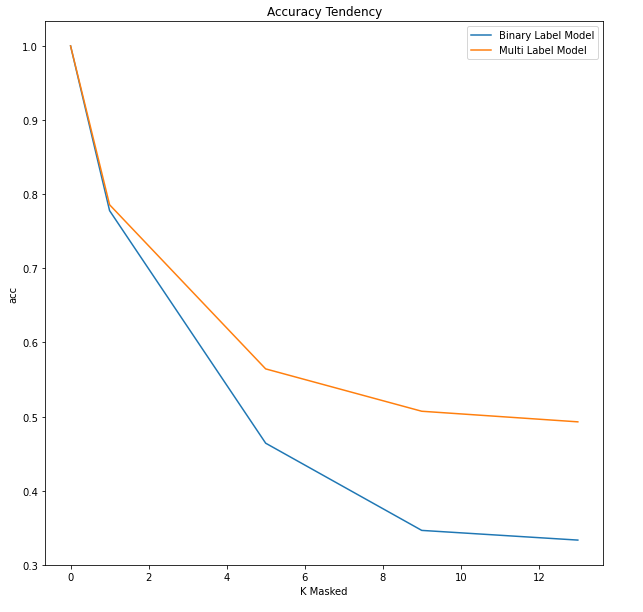
\includegraphics[width=0.7\textwidth]{Accuracy Tendency.png}
            \caption{Top K masked}
            \label{fig:MaskedExample}
    \end{figure}
\end{frame}

\begin{frame}
    \frametitle{Result}
    \framesubtitle{Accuracy Tendency}
    \begin{figure}
        \centering
            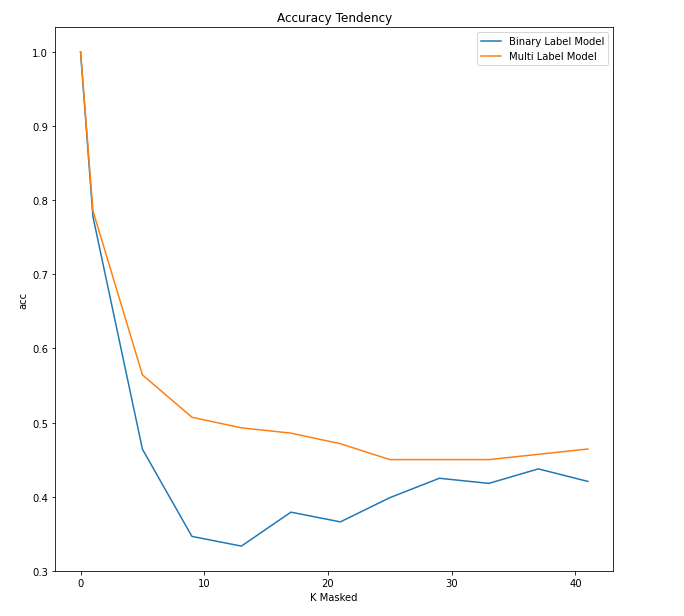
\includegraphics[width=0.7\textwidth]{Accuracy Tendency2.png}
            \caption{Top K masked}
            \label{fig:MaskedExample}
    \end{figure}
\end{frame}

\begin{frame}
    \frametitle{Code}
    \framesubtitle{Github Link: \\ $https:/github.com/RmmLeo/STAT6289_Homework/tree/main/Midterm\%20Project$}
    \begin{figure}
        \centering
            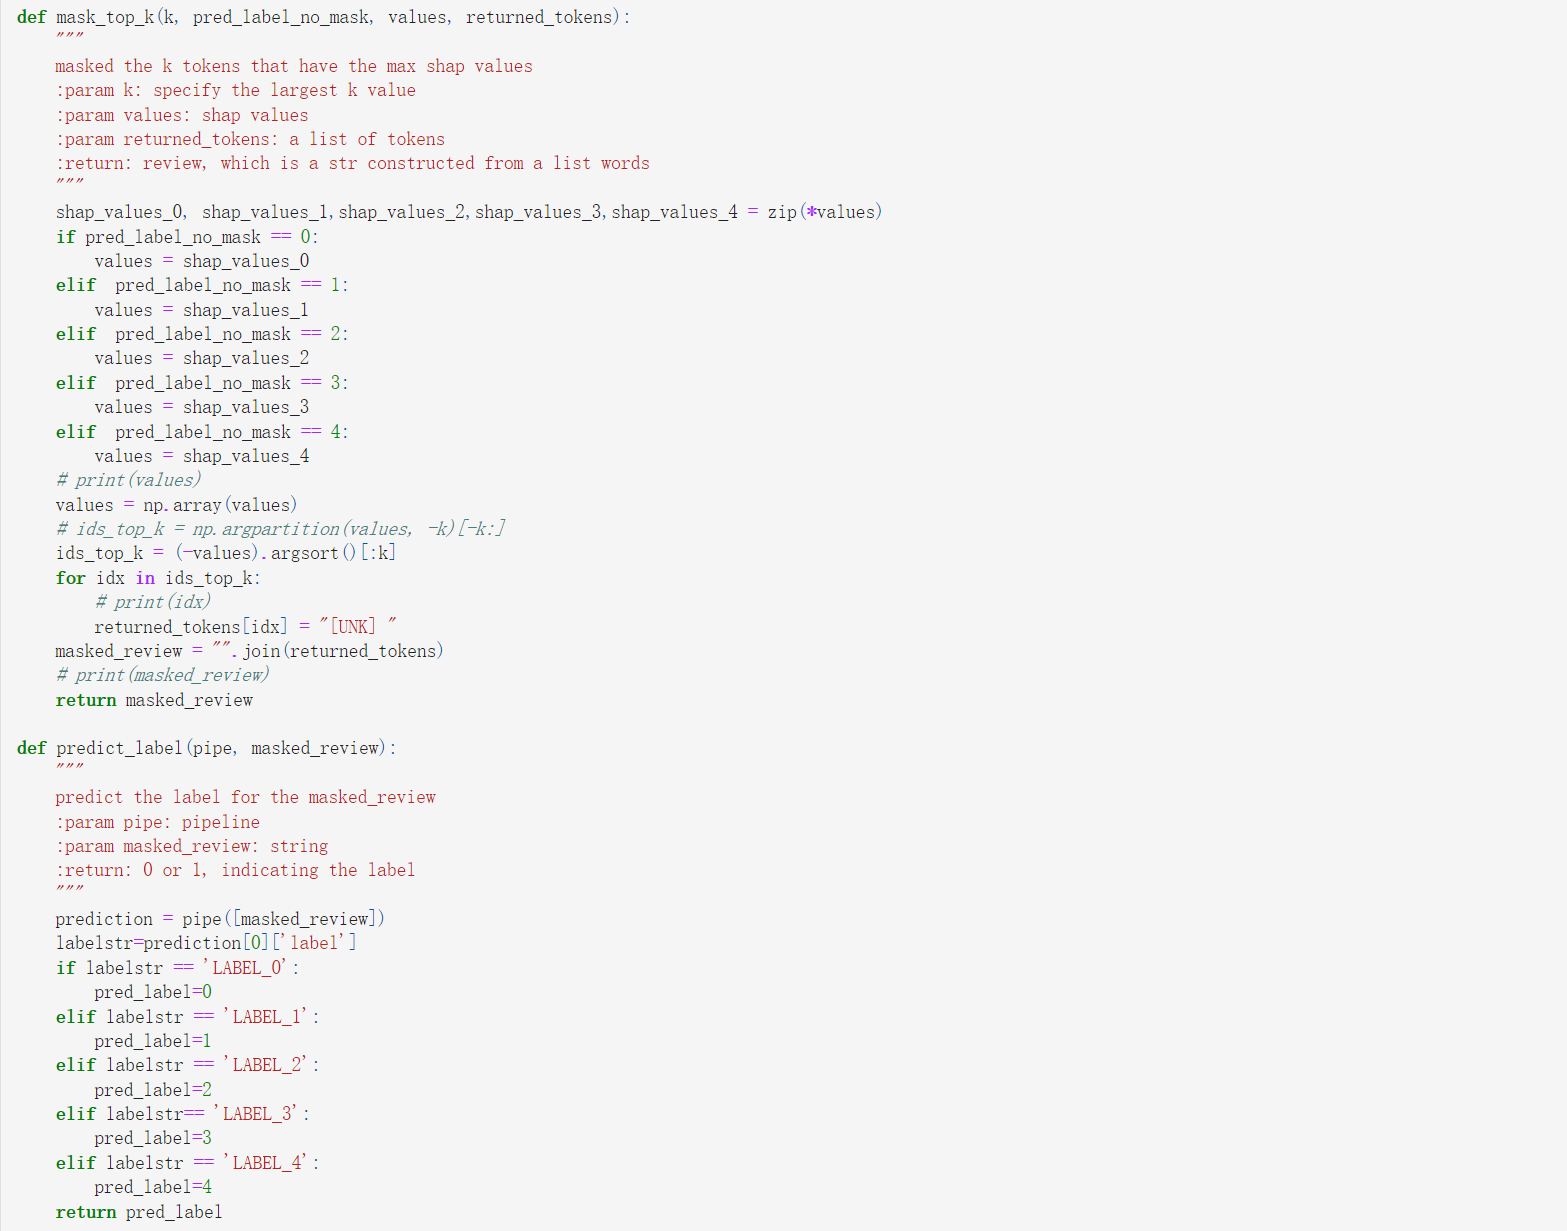
\includegraphics[width=0.7\textwidth]{Code1.png}
            \caption{Code1}
            \label{fig:MaskedExample}
    \end{figure}
\end{frame}

\begin{frame}
    \frametitle{Code}
    \begin{figure}
        \centering
            \includegraphics[width=0.7\textwidth]{Code2.png}
            \caption{Code2}
            \label{fig:MaskedExample}
    \end{figure}
\end{frame}
\end{document}